% begin module orthogonal-trajectory-def
\begin{frame}
\frametitle{Orthogonal Trajectories}
\begin{definition}[Orthogonal Trajectory]
An orthogonal trajectory to a family of curves is a curve that intersects each curve of the family orthogonally (that is, at right angles).
\end{definition}

\begin{columns}[c]
\column{.5\textwidth}
\psset{xunit=1cm, yunit=1cm}
\begin{pspicture}(-1.649994, -1.649998)(1.65,1.749998) 
\tiny 
\psaxesStandard{-1.399994}{-1.399998}{1.4}{1.399998}

%Calculator input: plotCurve{}(5/4 \cos{}t, 5/4 \sin{}t, 0, 2 \pi)
\parametricplot[linecolor=\psColorGraph, plotpoints=1000]{0}{6.28319}{t 57.29578 mul cos 1.25 mul t 57.29578 mul sin 1.25 mul }

%Calculator input: plotCurve{}(\cos{}t, \sin{}t, 0, 2 \pi)
\parametricplot[linecolor=\psColorGraph, plotpoints=1000]{0}{6.28319}{t 57.29578 mul cos t 57.29578 mul sin }

%Calculator input: plotCurve{}(3/4 \cos{}t, 3/4 \sin{}t, 0, 2 \pi)
\parametricplot[linecolor=\psColorGraph, plotpoints=1000]{0}{6.28319}{t 57.29578 mul cos 0.75 mul t 57.29578 mul sin 0.75 mul }

\psline[linecolor=blue] (1.293431, 0.535757) (-1.293431, -0.535757)
\psline[linecolor=blue] (0.989949, 0.989949) (-0.989949, -0.989949)
\psline[linecolor=blue] (0.535757, 1.293431) (-0.535757, -1.293431)
\psline[linecolor=blue] (-0.535757, 1.293431) (0.535757, -1.293431)
\psline[linecolor=blue] (-0.989949, 0.989949) (0.989949, -0.989949)
\psline[linecolor=blue] (-1.293431, 0.535757) (1.293431, -0.535757)
\end{pspicture} 

%\ \uncover<2->{%
%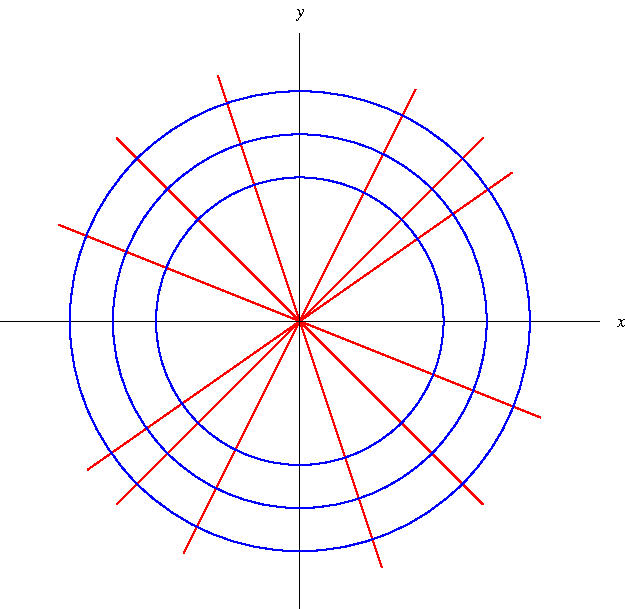
\includegraphics[height=5.5cm]{diff-eq-separable/pictures/10-03-orthcirc.pdf}%
%}%
\column{.5\textwidth}
\uncover<2->{%
Each member of the family $y = mx$ of straight lines passing through the origin is an orthogonal trajectory to the family $x^2 + y^2 = r^2$ of circles centered at the origin.
}%
\end{columns}
\end{frame}
% end module orthogonal-trajectory-def
